
%%==================================================
%% Ma Thesis.tex for DUT Thesis
%% version: 1.2
%% last update: Apr 27th, 2022
%%==================================================


\documentclass[twoside,doctor,hide]{DUT-thesis-grd}



%==============更改数学字体设置,Latin Modern Math 默认的的确有点细,看个人需要,下面提供一种方法,需要的可以取消注释=========%

% \usepackage[bold-style=ISO]{unicode-math} %采用unicode-math,可以直接输入Unicode公式,当然传统的输入就行
% \setmathfont{XITS Math}  %目前unicode-math 支持几种数学字体,具体用法可以查看帮助文档,这里采用类似times字体科学数学字体,可以取消注释对比


\begin{document}

%%%%%%%%%%%%%%%%%%%%%%%%%%%%%%
%% 封面
%%%%%%%%%%%%%%%%%%%%%%%%%%%%%%

% 封面绘制
\maketitle


% 论文原创性声明和使用授权
\makeDeclareOriginal
%\addcontentsline{toc}{chapter}{大连理工大学学位论文版权使用授权书}


%%%%%%%%%%%%%%%%%%%%%%%%%%%%%%
%% 前置部分
%%%%%%%%%%%%%%%%%%%%%%%%%%%%%%
\frontmatter

% 摘要
%%==================================================
%% abstract.tex for DUT  Thesis
%% version: 0.1
%% last update: Apr 27th, 2022
%%==================================================

\begin{abstract}
大连理工大学硕士研究生撰写学位论文应当符合写作规范和排版格式的要求,以下格式为研究生院依据国家标准和行业规范所编制的硕士学位论文模板,供硕士研究生参照使用。\par 论文摘要是学位论文的缩影,文字要简练、明确。内容要包括目的、方法、结果和结论。单位制一律换算成国际标准计量单位制,除特殊情况外,数字一律用阿拉伯数码。文中不允许出现插图,重要的表格可以写入。\par  摘要的主要内容为,简述全文的目的和意义、采用方法、主要研究内容和结论。\par 篇幅以一页为限,摘要正文后列出3-5个关键词,关键词与摘要之间空一行。\par“关键词:”是关键词部分的引导,不可省略。\par 关键词请尽量用《汉语主题词表》等词表提供的规范词。关键词之间用分号间隔,末尾不加标点。


\keywords{写作规范;排版格式;硕士学位论文}
\end{abstract}

\begin{englishabstract}

Contents of the abstract.Times New Roman.
   
\englishkeywords{Write Criterion; Typeset Format; Master's Degree Thesis}

\end{englishabstract}

%% 符号对照表,可选,如不用可注释掉

% 加入目录
\tableofcontents

\tableofengcontents

%加入图、表索引(同时取消图表索引中章之间的垂直间隔)
\let\origaddvspace\addvspace
\renewcommand{\addvspace}[1]{}
\addcontentsline{toc}{chapter}{图目录}
\listoffigures
\addcontentsline{toc}{chapter}{表目录}
\listoftables
\renewcommand{\addvspace}[1]{\origaddvspace{#1}}


\begin{denotation}
	\vspace{-20pt}
\begin{center}
% Table generated by Excel2LaTeX from sheet 'Sheet1'
\begin{table}[htbp]
	\centering
	\begin{tabular}{rrrcccccccccccccrrr}
		\toprule
		&       &       & \multicolumn{3}{c}{\textbf{符  号}} &       & \multicolumn{4}{c}{\textbf{代表意义}} &       & \multicolumn{4}{c}{\textbf{单位或定义}} &       &       &  \\
		&       &       & \multicolumn{3}{c}{\textbf{英文字母}} &       & \multicolumn{4}{c}{}          &       & \multicolumn{4}{c}{}          &       &       &  \\
		&       &       & \multicolumn{3}{c}{\textit{A}} &       & \multicolumn{4}{c}{加热面面积}     &       & \multicolumn{4}{c}{$\rm{cm^2}$}       &       &       &  \\
		&       &       & \multicolumn{3}{c}{$A_{\rm{liquid}}$} &       & \multicolumn{4}{c}{加热面润湿区域}   &       & \multicolumn{4}{c}{$\rm{cm^2}$}       &       &       &  \\
		&       &       & \multicolumn{3}{c}{\textit{B}} &       & \multicolumn{4}{c}{热流密度决定性偏差} &       & \multicolumn{4}{c}{\textbackslash{}} &       &       &  \\
		&       &       & \multicolumn{3}{c}{Cp} &       & \multicolumn{4}{c}{比热容}       &       & \multicolumn{4}{c}{kJ/(kg·K)} &       &       &  \\
		\multicolumn{4}{c}{}          &       &
		\multicolumn{4}{c}{}          &       & \multicolumn{4}{c}{}          &       &       &  \\
		&       &       & \multicolumn{3}{c}{\textbf{无量纲量}} &       & \multicolumn{4}{c}{}          &       & \multicolumn{4}{c}{}          &       &       &  \\
		&       &       & \multicolumn{3}{c}{\textit{Re}} &       & \multicolumn{4}{c}{雷诺数}       &       & \multicolumn{4}{c}{}          &       &       &  \\
		&       &       & \multicolumn{3}{c}{}  &       & \multicolumn{4}{c}{斯特劳哈尔数}    &       & \multicolumn{4}{c}{}          &       &       &  \\
		&       &       & \multicolumn{3}{c}{}  &       & \multicolumn{4}{c}{韦伯数}       &       & \multicolumn{4}{c}{}          &       &       &  \\
		&       &       & \multicolumn{3}{c}{}  &       & \multicolumn{4}{c}{}          &       & \multicolumn{4}{c}{}          &       &       &  \\
		&       &       & \multicolumn{3}{c}{\textbf{希腊字母}} &       & \multicolumn{4}{c}{}          &       & \multicolumn{4}{c}{}          &       &       &  \\
		&       &       & \multicolumn{3}{c}{}  &       & \multicolumn{4}{c}{密度}        &       & \multicolumn{4}{c}{$\rm{kg/{m}^{3}}$}     &       &       &  \\
		&       &       & \multicolumn{3}{c}{}  &       & \multicolumn{4}{c}{黏度}        &       & \multicolumn{4}{c}{Pa$\cdot$s}      &       &       &  \\
		&       &       & \multicolumn{3}{c}{}  &       & \multicolumn{4}{c}{蒸发效率}      &       & \multicolumn{4}{c}{}          &       &       &  \\
		&       &       & \multicolumn{3}{c}{}  &       & \multicolumn{4}{c}{}          &       & \multicolumn{4}{c}{}          &       &       &  \\
		&       &       & \multicolumn{3}{c}{\textbf{下标}} &       & \multicolumn{4}{c}{}          &       & \multicolumn{4}{c}{}          &       &       &  \\
		&       &       & \multicolumn{3}{c}{0} &       & \multicolumn{4}{c}{x = 0 或 t = 0} &       & \multicolumn{4}{c}{}          &       &       &  \\
		&       &       & \multicolumn{3}{c}{sat} &       & \multicolumn{4}{c}{饱和态}       &       & \multicolumn{4}{c}{}          &       &       &  \\
		&       &       & \multicolumn{3}{c}{}  &       & \multicolumn{4}{c}{}          &       & \multicolumn{4}{c}{}          &       &       &  \\
		&       &       & \multicolumn{3}{c}{\textbf{缩写}} &       & \multicolumn{4}{c}{}          &       & \multicolumn{4}{c}{}          &       &       &  \\
		&       &       & \multicolumn{3}{c}{CHF} &       & \multicolumn{4}{c}{临界热流密度}    &       & \multicolumn{4}{c}{}          &       &       &  \\
		&       &       & \multicolumn{3}{c}{IHCP} &       & \multicolumn{4}{c}{导热逆问题}     &       & \multicolumn{4}{c}{}          &       &       &  \\
		&       &       & \multicolumn{3}{c}{SFSM} &       & \multicolumn{4}{c}{顺序函数法}     &       & \multicolumn{4}{c}{}          &       &       &  \\
		\bottomrule
	\end{tabular}%
	\label{tab:addlabel}%
\end{table}%
\vspace{-10pt}
\hspace{-68pt}
\textbf{注:如文中对符号另有说明,以文中对应位置说明为准。}



\end{center}
\end{denotation}



%%%%%%%%%%%%%%%%%%%%%%%%%%%%%%
%% 正主体部分
%%%%%%%%%%%%%%%%%%%%%%%%%%%%%%
\mainmatter

%% 各章正文内容
\let\cleardoublepage\clearpage
%%==================================================
%% chapter01.tex for DUT Thesis 
%% version: 0.1
%% last update: Dec 25th, 2022
%%==================================================
\BiChapter{绪论}{Introduction}
绪论应包括本研究课题的学术背景及其理论与实际意义;本领域的国内外研究进展及成果、存在不足或有待深入研究的问题;本研究课题的来源及主要研究内容等。
\label{chap:intro}
\BiSection{研究背景与意义}{Research background}

\BiSection{国内外相关研究工作进展}{Research progress}

\BiSection{论文研究思路及目标}{Main research contents and objectives}





\BiChapter{Latex模板简介}{The Introduction of Latex Template}
本章介绍Latex的文本控制流程,介绍学位论文中各章节分布及模板内部组成,用户可根据自身对Latex的熟悉程度适当地略过阅读。\par
\BiSection{认识模板组成}{Understanding Template Composition}
格式控制文件控制着论文的表现形式,包括以下两个后缀的文件:“.cls”后缀的文件控制论文主体格式和“.bst”后缀的文件控制参考文献条目。\par
一般用户在.cls后缀的文件里填写封面、申明和授权书及奇偶页页眉内容,然后在各章正文处进行内容的填写。
\BiSection{主控文件}{Main File}
主控文件MA Thesis.tex的作用就是将分散在多个文件中的内容整合成一篇完整的内容。此部分用户不需做改动。
\BiSection{论文主体文件夹chapters}{Chapters File}
这一部分是论文的主体,是以“章”为单位划分的。用户需要在这里对中英文摘要、符号表、各章内容、附录、致谢、攻读学位论文期间的成果及作者简介进行填写。
\BiSection{图片文件夹figures}{Figures File}
figures文件夹放置了需要插入文档中的图片文件(PNG/JPG/PDF/EPS)。如果图片较多,建议按章再划分子目录存储图片。
\BiSection{参考文献数据库文件夹reference}{Reference File}
此文件夹用于存放参考文献信息。bib数据库中的参考文献条目可以手动编写,也可以在Google的学术搜索中找到。各大数据库也支持将参考文献信息导出为.bib。
\BiSection{本章小结}{The Chapter’s Conclusion}




\BiChapter{图表、公式、代码及参考文献的编制方法}{The Compile Method of Chart, Formula , Code and Reference }
\BiSection{向文档中插入图像}{Inserts an Image Into the Document}
\BiSubsection{单张图片的插入}{Insertion of a Single Image}
在学位论文中,可插入PDF、EPS、PNG、JPG格式的图片。以图3.1的插入为例,插入代码为3.1所示,其中\textbackslash centering表示图片居中,\textbackslash includegraphics[...]\{...\}导入图片并定制图片大小,\textbackslash\{...\}指定图片标题,而\textbackslash lable\{...\}为图片加上引用标签:
\begin{lstlisting}[caption={示例插图代码}]
\begin{figure}[!ht]
\centering
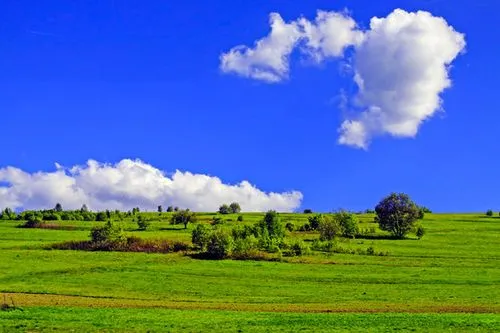
\includegraphics{figures/figure4}
\bicaption{图片}{Picture}  \label{fig4:diagram}
\end{figure}
\end{lstlisting}

\begin{figure}[!ht]
	\centering
	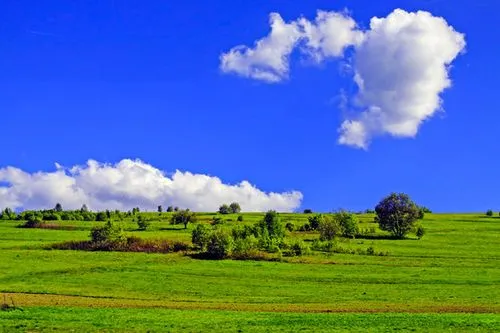
\includegraphics{figures/figure4}
	\bicaption{图片}{Picture}  \label{fig4:diagram}
\end{figure}
\BiSubsection{两张并列图片的插入}{The Insertion of Two Side-by-side Pictures}
插入两幅并列子图的例子如图3.2所示。这两个水平并列放置的图共享一个“图标题”,且有各自的小标题,并列子图的功能是使用subfigure宏包提供的。
\begin{lstlisting}[caption={插入并列子图代码}]
\begin{figure}[!ht]
\centering
\subfigure[热流耦合数值模拟]{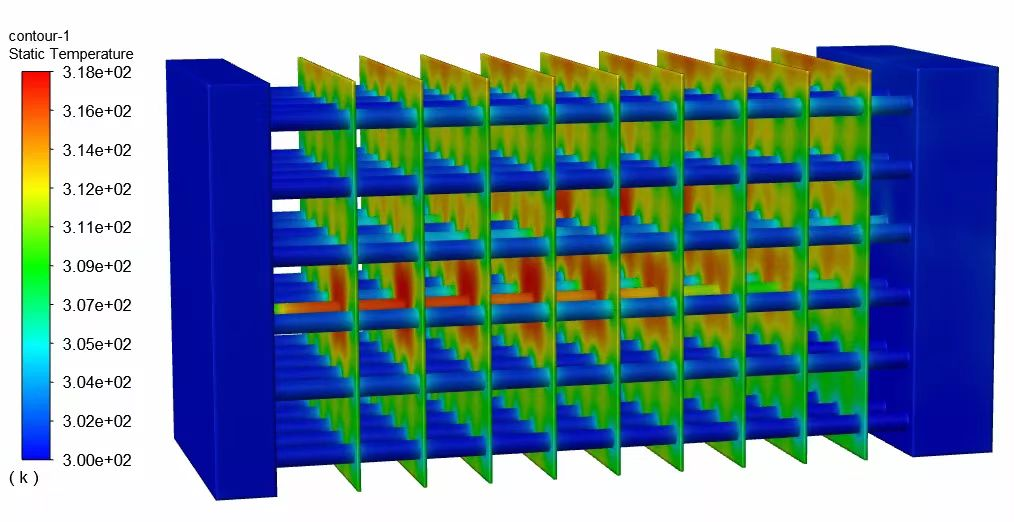
\includegraphics[width=0.45\textwidth]{figures/figure8}}
\subfigure[热固耦合数值模拟]{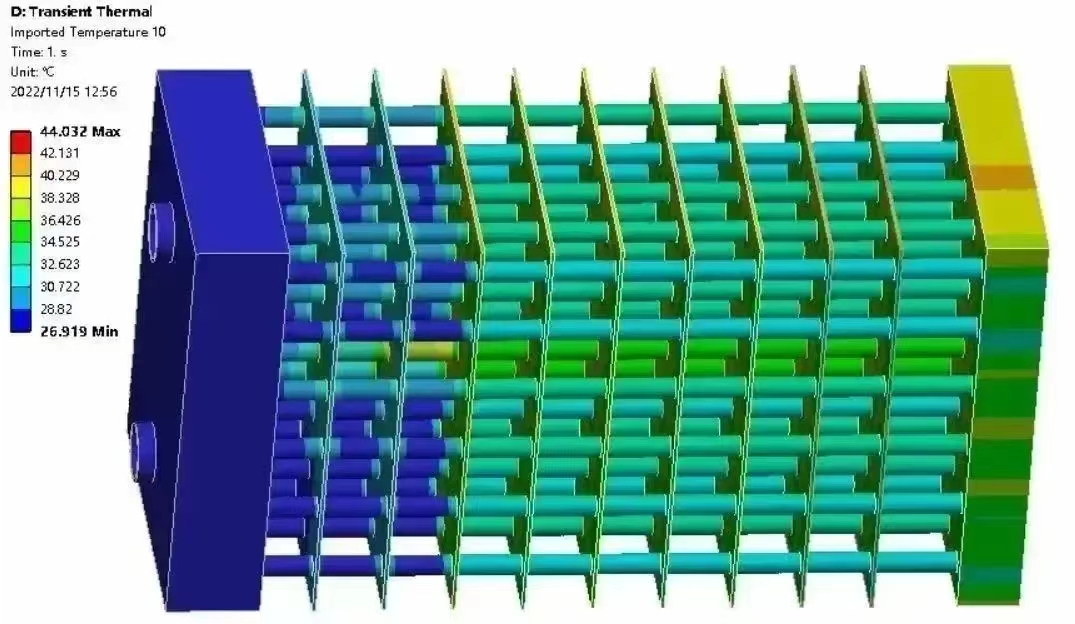
\includegraphics[width=0.45\textwidth]{figures/figure9}}
\bicaption{数值模拟图像}{Numerical simulation image}
\end{figure}
\end{lstlisting}
\begin{figure}[!ht]
	\centering
	\subfigure[热流耦合数值模拟]{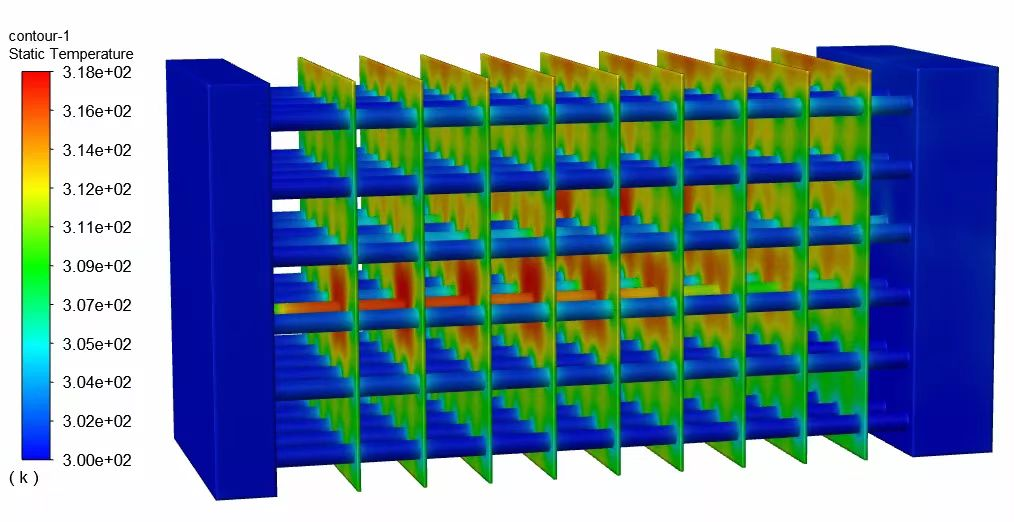
\includegraphics[width=0.45\textwidth]{figures/figure8}}
	\subfigure[热固耦合数值模拟]{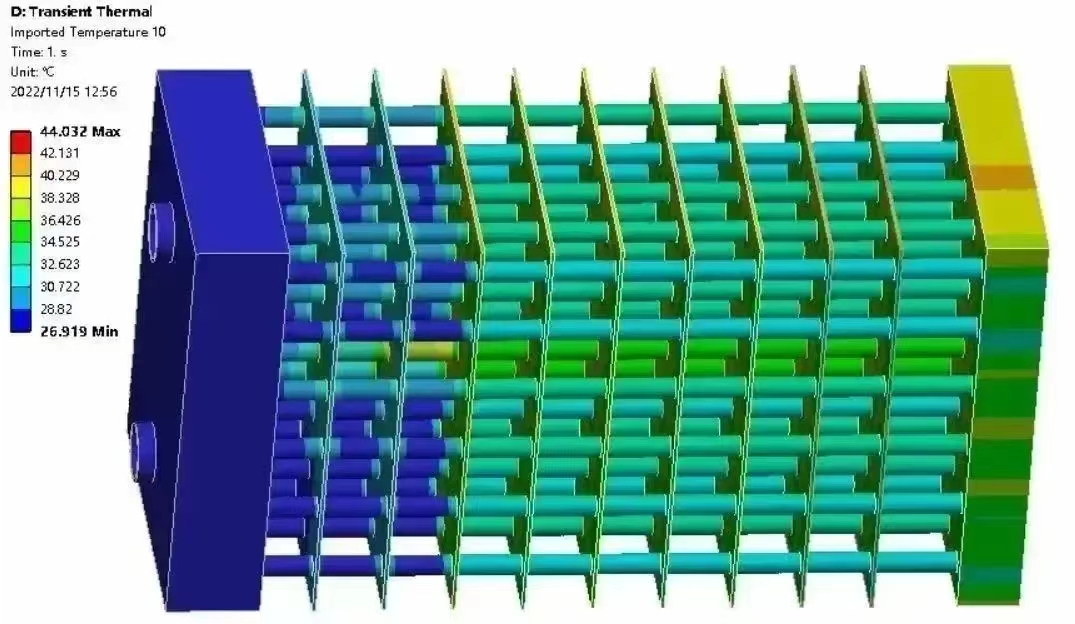
\includegraphics[width=0.45\textwidth]{figures/figure9}}
	\bicaption{数值模拟图像}{Numerical simulation image}
\end{figure}
更多关于Latex插图的例子可以参考《\LaTeX 插图指南》。
\BiSection{表格的例子}{Example of Table Compile}
表在正文中的常用格式如表\ref{tab3:category},使用三线表。\par
\begin{table}[!ht]
	\small
	\centering
	\bicaption{国内外各返回式航天器热控设计情况}{ Design of thermal control systems of spacecraft for different countries} \label{tab3:category}
	\begin{tabular}{m{5em}<{\centering}m{5em}<{\centering}m{5em}<{\centering}m{5em}<{\centering}m{5em}<{\centering}m{5em}<{\centering}}
		\toprule[2pt]
		项目、指标 &月地高速再入返回器&传统返回式卫星回收舱&神舟飞船&国外载人飞船&航天飞机 \\
		\midrule[1pt]
		回收舱气密性&半密封舱&非密封舱&密封舱&密封舱&密封舱\\
		回收舱长期热耗(W)&整器150&5 – 25&约1000(含宇航员)&约1000(含宇航员)&1500以上\\
		热控方案&基于柔性自适应“热开关”的新型热控方案&被动热控设计为主、电加热主动热控设计为辅&泵驱单相流体回路+对流通风&泵驱单相流体回路+对流通风&泵驱单相流体回路+对流通风+主动式相变系统\\
		\bottomrule[2pt]
	\end{tabular}
\end{table}
表格的绘制需要知道一些基本命令的用法,比如“\&”具有对齐作用,\textbackslash multicolumn用来合并行,\textbackslash multirow用来合并列,\textbackslash hline表示加入横线进行分隔,还有许多命令这里就不一一展开说明,这里给出一些表格绘制的例子进行示范:
\begin{lstlisting}[caption={表3.2绘制代码}]
\begin{table}[!ht]
\small
\centering
\bicaption{国际单位制的辅助单位况}{ Assistant units of International System of Units} 
\begin{tabular}{m{6em}<{\centering}m{6em}<{\centering}m{6em}<{\centering}}
\toprule[2pt]
量的名称&单位名称&单位符号 \\
\midrule[1pt]
平面角&弧度&rad\\
立体角&球面度&sr\\
\bottomrule[2pt]
\end{tabular}
\end{table}
\end{lstlisting}
\begin{table}[!ht]
	\small
	\centering
	\bicaption{国际单位制的辅助单位况}{ Assistant units of International System of Units} 
	\begin{tabular}{m{6em}<{\centering}m{6em}<{\centering}m{6em}<{\centering}}
		\toprule[2pt]
		量的名称&单位名称&单位符号 \\
		\midrule[1pt]
		平面角&弧度&rad\\
		立体角&球面度&sr\\
		\bottomrule[2pt]
	\end{tabular}
\end{table}
\begin{lstlisting}[caption={表3.3绘制代码}]
\begin{table}[!ht]
\small
\centering
\bicaption{国际单位制中具有专门名称的导出单位}{Export units of special name in International System of Units} 
\begin{tabular}{m{8em}<{\centering}m{6em}<{\centering}m{4em}<{\centering}m{6em}<{\centering}} 
\toprule[2pt]
量的名称&单位名称&单位符号&其他表示式例 \\
\midrule[1pt]
频率&赫[兹]&Hz&$\rm{s^{-1}}$\\
力;重力&牛[顿]&N&$\rm{kg·m/s^2}$\\
压力,压强;应力&	帕[斯卡]&	Pa&$\rm{N/m^2}$\\
能量;功;热	&焦[耳]&	J&	N·m\\
功率;辐射通量&	瓦[特]&	W&	J/s\\
电荷量	&库[仑]&	C&	A·s\\
电位;电压;电动势&	伏[特]&	V&	W/A\\
电容&	法[拉]&	F&	C/V\\
电阻&	欧[姆]&	Ω&	V/A\\
电导&	西[门子]&	S&	A/V\\
磁通量	&韦[伯]&	Wb&	V·s\\
磁通量密度,磁感应强度	&特[斯拉]&	T&$	\rm{Wb/m^2}$\\
电感&	亨[利]&	H&	Wb/A\\
摄氏温度&	摄氏度&	℃	&   \\
光通量&	流明&	lm&	cd·sr\\
光照度	&勒[克斯]&	lx&	$\rm{lm/m^2}$\\
放射性活度&	贝可[勒尔]&	Bq&$\rm{s^{-1}}$\\
吸收剂量&	戈[瑞]&	Gy&	J/kg\\
剂量当量&	希[沃特]&	Sv&	J/kg\\
\bottomrule[2pt]
\end{tabular}
\end{table}
\end{lstlisting}
\begin{table}[!ht]
	\small
	\centering
	\bicaption{国际单位制中具有专门名称的导出单位}{Export units of special name in International System of Units} 
	\begin{tabular}{m{8em}<{\centering}m{6em}<{\centering}m{4em}<{\centering}m{6em}<{\centering}} 
		\toprule[2pt]
		量的名称&单位名称&单位符号&其他表示式例 \\
		\midrule[1pt]
		频率&赫[兹]&Hz&$\rm{s^{-1}}$\\
		力;重力&牛[顿]&N&$\rm{kg·m/s^2}$\\
		压力,压强;应力&	帕[斯卡]&	Pa&$\rm{N/m^2}$\\
		能量;功;热	&焦[耳]&	J&	N·m\\
		功率;辐射通量&	瓦[特]&	W&	J/s\\
		电荷量	&库[仑]&	C&	A·s\\
		电位;电压;电动势&	伏[特]&	V&	W/A\\
		电容&	法[拉]&	F&	C/V\\
		电阻&	欧[姆]&	Ω&	V/A\\
		电导&	西[门子]&	S&	A/V\\
		磁通量	&韦[伯]&	Wb&	V·s\\
		磁通量密度,磁感应强度	&特[斯拉]&	T&$	\rm{Wb/m^2}$\\
		电感&	亨[利]&	H&	Wb/A\\
		摄氏温度&	摄氏度&	℃	&   \\
		光通量&	流明&	lm&	cd·sr\\
		光照度	&勒[克斯]&	lx&	$\rm{lm/m^2}$\\
		放射性活度&	贝可[勒尔]&	Bq&$\rm{s^{-1}}$\\
		吸收剂量&	戈[瑞]&	Gy&	J/kg\\
		剂量当量&	希[沃特]&	Sv&	J/kg\\
		\bottomrule[2pt]
	\end{tabular}
\end{table}
\begin{lstlisting}[caption={表3.4绘制代码}]
\begin{table}[!ht]
\small
\centering
\bicaption{国际单位制的基本单位}{ Basic units of International System of Units} 
\begin{tabular}{m{6em}<{\centering}m{6em}<{\centering}m{6em}<{\centering}}
\toprule[2pt]
量的名称&单位名称&单位符号 \\
\midrule[1pt]
长度	&米&	m\\
质量&	千克(公斤)&	kg\\
时间&	秒&	s\\
电流&	安[培]&	A\\
热力学温度&	开[尔文]&	K\\
物质的量&	摩[尔]&	mol\\
发光强度&	坎[德拉]&	cd\\
\bottomrule[2pt]
\end{tabular}
\end{table}
\end{lstlisting}
\begin{table}[!ht]
	\small
	\centering
	\bicaption{国际单位制的基本单位}{ Basic units of International System of Units} 
	\begin{tabular}{m{6em}<{\centering}m{6em}<{\centering}m{6em}<{\centering}}
		\toprule[2pt]
		量的名称&单位名称&单位符号 \\
		\midrule[1pt]
		长度	&米&	m\\
		质量&	千克(公斤)&	kg\\
		时间&	秒&	s\\
		电流&	安[培]&	A\\
		热力学温度&	开[尔文]&	K\\
		物质的量&	摩[尔]&	mol\\
		发光强度&	坎[德拉]&	cd\\
		\bottomrule[2pt]
	\end{tabular}
\end{table}
\begin{lstlisting}[caption={表3.5绘制代码}]
\begin{table}[!ht]
\small
\centering
\bicaption{国家选定的非国际单位制单位}{Non-International System of Units adopted by the nation} 
\begin{tabular}{m{5em}<{\centering}m{7em}<{\centering}m{5em}<{\centering}m{11em}<{\centering}m{5em}<{\centering}m{5em}<{\centering}}
\toprule[2pt]
量的名称&	单位名称&	单位符号&	换算关系和说明 \\
\midrule[1pt]
\multirow{3}*{时间}&分&min&1 min = 60 s\\
&[小]时&	h&1 h = 60 min= 3600 s\\
&天(日)&d	&	1 d = 24 h= 86400 s\\
\multirow{3}*{平面角}&[角]秒&(")&1" = (π / 648000) rad\\
&[角]分&(')&1' = 60"= (π / 10800) rad\\
&度&(°)	&	1 ° = 60' = (π / 180) rad\\
旋转速度&	转每分&	r/min&	1 r/min = (1 / 60)$\rm{s^{-1}}$\\
\multirow{2}*{长度}&\multirow{2}*{海里}&\multirow{2}*{n mile}&
mile = 1852 m\\&&&(只用于航行)\\
\multirow{3}*{速度}&\multirow{3}*{节}&\multirow{3}*{kn}&
1 kn=1 n mile/h\\&&&= (1852 / 3600) m/s\\&&&(只用于航行)\\
\multirow{2}*{质量}&吨&t&1 t=$10^3$ kg\\
&原子质量单位&u&1 u≈1.6605655 × $10^{-27}\rm{kg}$\\
体积&	升&	L,(1)&	1 L = $10^{-3}\rm{ m^3}$\\
能&	电子伏&	eV&	1 eV≈1.6021892 × $10^{-19}$J\\
级差	&分贝&	dB	&\\
级密度	&特[克斯]&	tex&	1 tex=1 g/km\\	
\bottomrule[2pt]
\end{tabular}
\end{table}
\end{lstlisting}
\begin{table}[!ht]
	\small
	\centering
	\bicaption{国家选定的非国际单位制单位}{Non-International System of Units adopted by the nation} 
	\begin{tabular}{m{5em}<{\centering}m{7em}<{\centering}m{5em}<{\centering}m{11em}<{\centering}m{5em}<{\centering}m{5em}<{\centering}}
		\toprule[2pt]
		量的名称&	单位名称&	单位符号&	换算关系和说明 \\
		\midrule[1pt]
		\multirow{3}*{时间}&分&min&1 min = 60 s\\
		&[小]时&	h&1 h = 60 min= 3600 s\\
		&天(日)&d	&	1 d = 24 h= 86400 s\\
		\multirow{3}*{平面角}&[角]秒&(")&1" = (π / 648000) rad\\
		&[角]分&(')&1' = 60"= (π / 10800) rad\\
		&度&(°)	&	1 ° = 60' = (π / 180) rad\\
		旋转速度&	转每分&	r/min&	1 r/min = (1 / 60)$\rm{s^{-1}}$\\
		\multirow{2}*{长度}&\multirow{2}*{海里}&\multirow{2}*{n mile}&
		mile = 1852 m\\&&&(只用于航行)\\
		\multirow{3}*{速度}&\multirow{3}*{节}&\multirow{3}*{kn}&
		1 kn=1 n mile/h\\&&&= (1852 / 3600) m/s\\&&&(只用于航行)\\
		\multirow{2}*{质量}&吨&t&1 t=$10^3$ kg\\
		&原子质量单位&u&1 u≈1.6605655 × $10^{-27}\rm{kg}$\\
		体积&	升&	L,(1)&	1 L = $10^{-3}\rm{ m^3}$\\
		能&	电子伏&	eV&	1 eV≈1.6021892 × $10^{-19}$J\\
		级差	&分贝&	dB	&\\
		级密度	&特[克斯]&	tex&	1 tex=1 g/km\\	
		\bottomrule[2pt]
	\end{tabular}
\end{table}
\begin{lstlisting}[caption={表3.6绘制代码}]
\begin{table}[!ht]
\small
\centering
\bicaption{用于构成十进倍数和分数单位的词头}{ Used prefixes to make up of denary multiples and subdivisions of the units} 
\begin{tabular}{m{6em}<{\centering}m{6em}<{\centering}m{6em}<{\centering}}
\toprule[2pt]
所表示的因数&	词头名称&	词头符号\\
\midrule[1pt]
$\rm10^{18}$&	艾[克萨]&	E\\
$\rm10^{15}$&	拍[它]&	P\\
$\rm10^{12}$&	太[拉]&	T\\
$\rm10^9$&	吉[咖]&	G\\
$\rm10^6$	&兆&	M\\
$\rm10^3$&	千&	K\\
$\rm10^2$&	百&	h\\
$\rm10^1$	&十&	da\\
$\rm10^{-1}$&	分&	d\\
$\rm10^{-2}$&	厘&	c\\
$\rm10^{-3}$&	毫&	m\\
$\rm10^{-6}$&	微&	μ\\
$\rm10^{-9}$&	纳[诺]&	n\\
$\rm10^{-12}$&	皮[可]&	p\\
$\rm10^{-15}$&	飞[母托]&	f\\
$\rm10^{-18}$&	阿[托]&	a\\	
\bottomrule[2pt]
\end{tabular}
\end{table}
\end{lstlisting}
\begin{table}[!ht]
	\small
	\centering
	\bicaption{用于构成十进倍数和分数单位的词头}{ Used prefixes to make up of denary multiples and subdivisions of the units} 
	\begin{tabular}{m{6em}<{\centering}m{6em}<{\centering}m{6em}<{\centering}}
		\toprule[2pt]
		所表示的因数&	词头名称&	词头符号\\
		\midrule[1pt]
		$\rm10^{18}$&	艾[克萨]&	E\\
		$\rm10^{15}$&	拍[它]&	P\\
		$\rm10^{12}$&	太[拉]&	T\\
		$\rm10^9$&	吉[咖]&	G\\
		$\rm10^6$	&兆&	M\\
		$\rm10^3$&	千&	K\\
		$\rm10^2$&	百&	h\\
		$\rm10^1$	&十&	da\\
		$\rm10^{-1}$&	分&	d\\
		$\rm10^{-2}$&	厘&	c\\
		$\rm10^{-3}$&	毫&	m\\
		$\rm10^{-6}$&	微&	μ\\
		$\rm10^{-9}$&	纳[诺]&	n\\
		$\rm10^{-12}$&	皮[可]&	p\\
		$\rm10^{-15}$&	飞[母托]&	f\\
		$\rm10^{-18}$&	阿[托]&	a\\	
		\bottomrule[2pt]
	\end{tabular}
\end{table}
\BiSection{公式的插入}{The Insertion of Formula}
公式的输入非常简单,只要在以下代码的相应位置改成自己要输入的公式即可。
\begin{lstlisting}[caption={公式插入代码}]
\begin{equation}
St=\frac{fd}{v}=\frac{f\overline{d_{32}}}{\overline{Q^{''}}}
\label{eq:St}
\end{equation}
\end{lstlisting}
\begin{equation}
St=\frac{fd}{v}=\frac{f\overline{d_{32}}}{\overline{Q^{''}}}
\label{eq:St}
\end{equation}



\BiSection{参考文献管理}{Reference Management}
参考文献的具体内容就是 reference 文件夹下的 .bib,参考文献的元数据 (名称、作者、出处等) 以一定的格式保存在这些纯文本文件中。.bib 文件也可以理解为参考文献的“数据库”,正文中所有引用的参考文件条目都会从这些文件中“析出”。控制参考文献条目“表现形式”(格式) 的是.bst 文件。.bst 文件定义了参考文献风格,使用不同的参考文献风格能将同一个参考文献条目输出成不同的格式。当然,一个文档只能使用一个参考文献风格。按照学校要求,本模板使用的是国标 GBT7714 风格的参考文献。
\BiSubsection{Latex中参考文献的引用与插入方法}{Citation and Insertion of References in Latex}
bib数据库中的参考文献条目可以手动编写,也可以在 Google 的学术搜索中找到。各大数据库也支持将参考文献信息导出为.bib,省时省力。以 Google 学术搜索为例:在“学术搜索设置”中,将“文献管理软件”设为“显示导入 BibTeX”的连接,保存退出。然后学术搜索找到文献后会有“导出到BibTeX”连接,点击后会打开新的标签页。插入文献详细的介绍点击链接\url{https://b23.tv/G1oMWUA},从22:48时开始是讲述怎么插入参考文献的。\par
其中需要注意的是由于中英文参考文献处理起来有差异,所以需要在参考文献中标注是否是中文文献。确切地说,BibTeX并不具有区分中英文参考文献的能力。.bib是“参考文献的内容”,而控制参考文献格式的是.bst文件,本模板附带的是GBT7714-2005NLang.bst。GBT7714-2005NLang.bst中规定:.bib中的条目,如果条目的“Language”域非空,就被认为是中文参考文献,采取一些针对中文的处理方式。\par
例如在如下一段话中插入参考文献,用\textbackslash cite\{文献标识\}在文中引用文献:
关于主题法的起源众说不一。国内有人认为“主题法检索体系的形式和发展开始于1856年英国克雷斯塔多罗(Crestadoro)的《图书馆编制目录技术》一书”,“国外最早采用主题法来组织目录索引的是杜威十进分类法的相关主题索引……” \cite{Jiang2005Size}。也有人认出为“美国的贝加逊·富兰克林出借图书馆第一个使用了主题法”\cite{Takahashi1996Structure,Xia2002Analysis,Jiang1989}。

\BiSection{定理与定义}{Definition and Proof}
定理与定义的写入很简单,方法如下:
\begin{lstlisting}[caption={定理写入代码}]
\begin{thm}
设函数$y=f(x)$在区间(a,b)上可导,它对应曲线是向上凹(或向下凹)的充分必要条件是:导数 $y=f^{'}(x)$在区间(a,b)上是单调增(或单调减)。
\end{thm}
\end{lstlisting}
\begin{thm}
	设函数$y=f(x)$在区间(a,b)上可导,它对应曲线是向上凹(或向下凹)的充分必要条件是:导数 $y=f^{'}(x)$在区间(a,b)上是单调增(或单调减)。
\end{thm}
\begin{lstlisting}[caption={定义写入代码}]
\begin{defn}[函数极值]
设函数$f(x)$在区间(a,b)内有定义,$x_0$是(a,b)内一点。\par
若存在着$x_0$点的一个邻域,对于这个邻域内任何点$x$($x_0$点除外),$f(x)<f(x_{0})$均成立,则说$f(x_{0})$ 是函数 $f(x)$的一个极大值;若存在着$x_0$点的一个邻域,对于这个邻域内任何点$x$($x_0$点除外),$f(x)>f(x_{0})$均成立,则说$f(x_{0})$ 是函数$f(x)$ 的一个极小值. 函数的极大值与极小值统称为函数的极值。
\end{defn}
\end{lstlisting}
\begin{defn}[函数极值]
	设函数$f(x)$在区间(a,b)内有定义,$x_0$是(a,b)内一点。\par
	若存在着$x_0$点的一个邻域,对于这个邻域内任何点$x$($x_0$点除外),$f(x)<f(x_{0})$均成立,则说$f(x_{0})$ 是函数 $f(x)$的一个极大值;若存在着$x_0$点的一个邻域,对于这个邻域内任何点$x$($x_0$点除外),$f(x)>f(x_{0})$均成立,则说$f(x_{0})$ 是函数$f(x)$ 的一个极小值. 函数的极大值与极小值统称为函数的极值。
\end{defn}

\BiSection{算法代码的插入}{Code Insertion Method}
论文中算法代码的插入示例如下:
\begin{lstlisting}[caption={算法代码的插入示例}]
\begin{algorithm}[h]  
   \caption{Pseudocode of Simulated Annealing Algorithm} % 名称 
   \begin{algorithmic}[1]   
     \Require      
       $x_0$: initial individual or state;     
       $T_0$: a high enough initial temperature;      
       $T_{min}$: the lowest limit of temperature;    
     \Ensure       
       optimal state or approximate optimal state;       
       \State set $x_0 = x_{best}$, compute initial energy function $E(x_0)$;       
       \While {$T > T_{min}$}        
        \For{$i = 1$; $i<n$; $i++$ }      
       \State perturb current state $x_i$ for a new state $x_{new}$ and compute energy function $E(x_{new})$;      
       \State compute $\Delta$ = $E(x_{new}-E(x_{(i)}))$;      
       \If {$\Delta$$E<0$} \State $x_{best} = x_{new}$      
       \Else \State the probability $P = exp(-dE/T_{(i)})$;      
       \If {$rand(0,1) < P$ }\State $x_{best} = x_{new}$      
       \Else \State $x_{best} = x_{best}$      
       \EndIf     
      \EndIf     
      \EndFor      
       \State $T = T * $ $ \alpha$, where $\alpha$ is decay factor;
     \EndWhile  
   \end{algorithmic}
\end{algorithm}
\end{lstlisting}

\begin{algorithm}[h]  
	\caption{Pseudocode of Simulated Annealing Algorithm} % 名称 
	\begin{algorithmic}[1]   
	  \Require      
		$x_0$: initial individual or state;     
		$T_0$: a high enough initial temperature;      
		$T_{min}$: the lowest limit of temperature;    
      \Ensure       
		optimal state or approximate optimal state;       
		\State set $x_0 = x_{best}$, compute initial energy function $E(x_0)$;       
		\While {$T > T_{min}$}        
		 \For{$i = 1$; $i<n$; $i++$ }      
		\State perturb current state $x_i$ for a new state $x_{new}$ and compute energy function $E(x_{new})$;      
		\State compute $\Delta$ = $E(x_{new}-E(x_{(i)}))$;      
		\If {$\Delta$$E<0$} \State $x_{best} = x_{new}$      
		\Else \State the probability $P = exp(-dE/T_{(i)})$;      
		\If {$rand(0,1) < P$ }\State $x_{best} = x_{new}$      
		\Else \State $x_{best} = x_{best}$      
		\EndIf     
       \EndIf     
	   \EndFor      
		\State $T = T * $ $ \alpha$, where $\alpha$ is decay factor;
	  \EndWhile  
	\end{algorithmic}
\end{algorithm}
\BiSection{规范表达注意事项}{The Standard Expression}
\BiSubsection{名词术语}{Terminology}
应使用全国自然科学名词审定委员会审定的自然科学名词术语;应按有关的标准或规定使用工程技术名词术语;应使用公认共知的尚无标准或规定的名词术语。作者自拟的名词术语,在文中第一次出现时,须加注说明。表示同一概念或概念组合的名词术语,全文中要前后一致。外国人名可使用原文,不必译出。一般的机关、团体、学校、研究机构和企业等的名称,在论文中第一次出现时必须写全称。
\BiSubsection{数字}{Figures}
数字的使用必须符合新的国家标准GB/T15835-1995《出版物上数字用法的规定》。
\BiSubsection{外文字母}{Foreign Letters}
文中出现的易混淆的字母、符号以及上下标等,必须打印清楚或缮写工整。要严格区分外文字母的文种、大小写、正斜体和黑白体等,必要时用铅笔注明,尤其注意上下标字母的大小写、正斜体。\par
(1) 斜体\par
斜体外文字母用于表示量的符号,主要用于下列场合:\par
1) 变量符号、变动附标及函数。\par
2) 用字母表示的数及代表点、线、面、体和图形的字母。\par
3) 特征数符号,如Re(雷诺数)、Fo(傅里叶数)、Al(阿尔芬数)等。\par
4) 在特定场合中视为常数的参数。\par
5) 矢量、矩阵用黑体斜体。\par
(2) 正体\par
正体外文字母用于表示名称及与其有关的代号,主要用于下列场合:\par
1) 有定义的已知函数(例如sin, exp, ln等)。\par
2) 其值不变的数学常数(例如e=2.718 281 8…)及已定义的算子。\par
3) 法定计量单位、词头和量纲符号。\par
4) 数学符号。\par
5) 化学元素符号。\par
6) 机具、仪器、设备和产品等的型号、代号及材料牌号。\par
7) 硬度符号。\par
8) 不表示量的外文缩写字。\par
9) 表示序号的拉丁字母。\par
10) 量符号中为区别其它量而加的具有特定含义的非量符号下角标。
\BiSubsection{量和单位}{Quantities and Units}
文中涉及的量和单位一律采用新的国家标准GB3100~3102-93《量和单位》。\par
(1) 必须符合国家标准规定,不得使用已废弃的单位,如高斯(G和Gg) 、亩、克分子浓度(M)、当量能度(N)等。\par
(2) 量和单位不用中文名称,而用法定符号表示。
\BiSubsection{标量与向量}{The scalar and Vector}
标量要采用正体,而向量要采用黑体。
\BiSection{本章小结}{The Chapter’s Conclusion}

\BiChapter{打印说明}{The Instruction of Printing}
\BiSection{封页}{Cover Sheet}
\BiSubsection{封皮}{Envelope}
大连理工大学印刷厂统一制作。
\BiSubsection{封一}{The First Envelope}
可直接双面打印。
\BiSubsection{封二}{The second Envelope}
可直接双面打印。
\BiSection{中英文摘要}{The Abstract in Chinese and English}
\BiSubsection{中文摘要}{The Abstract in Chinese}
可直接双面打印。
\BiSubsection{英文摘要}{The Abstract in English}
可直接双面打印,注意控制目录首页为奇数页。
\BiSection{目录}{Contents}
如果是一页,单面打印;如果两页,双面打印;如果三页,第一、二页双面打印,第三页单面打印。总而言之保证下一节首页为奇数页。
\BiSection{正文}{The Text}
\BiSubsection{正文}{The Text}
正文从绪论开始到致谢结束,双面打印。
\BiSection{本章小结}{The Chapter's Conclusion}
\BiChapter{第五章题目}{The Fourth Chapter Title}
(黑体,小三,1.5倍行距,段后1行)
\BiSection{第一节题目}{The First Quarter Title}
(黑体,四号,1.5倍行距,段前0.5行)
\BiSubsection{第一节一级题目}{The First Quarter Level 1 title}
(黑体,小四,1.5倍行距,段前0.5行)\par
\BiSection{第二节题目}{The Second Quarter Title}
\BiSubsection{第二节一级题目}{The Second Quarter Level 1 title}
\BiSection{本章小结}{ The Chapter’s Conclusion}


\BiChapter{结论与展望}{Conclusions and Prospection}
该部分主要包括三个部分:“结论”、“创新点”和“展望”。
\BiSection{结论}{ Conclusions}
结论是理论分析和实验结果的逻辑发展,是整篇论文的归宿。结论是在理论分析、试验结果的基础上,经过分析、推理、判断、归纳的过程而形成的总观点。结论必须完整、准确、鲜明、并突出与前人不同的新见解。
\BiSection{创新点}{Highlights}
创新点应该以分条列举的形式进行提出。\par
(1) 以预报……模型,建立了….。 \par
(2) 应用……方法,对颗粒受力情况进行了分析。\par
(3) ……\par
(4) ……
\BiSection{展望}{Prospection}
展望是对该研究课题存在的不足和有待改进的说明,是对未来研究的一种期待。




%% 参考文献,五号字,使用 BibTeX,包含参考文献文件.bib

%\bibliography{reference/chap1,reference/chap2} %多个章节的参考文献
\bibliography{reference/chap1}


%%%%%%%%%%%%%%%%%%%%%%%%%%%%%%
%% 后置部分
%%%%%%%%%%%%%%%%%%%%%%%%%%%%%%

%% 附录(章节编号重新计算,使用字母进行编号)
\appendix
\renewcommand{\appendixname}{附录~\Alph{chapter}}
\CTEXsetup[name={附录}]{chapter}
 % 附录中编号形式是"A.1"的样子
\renewcommand\thefigure{\Alph{chapter}.\arabic{figure}}
\renewcommand\thetable{\Alph{chapter}.\arabic{table}}
\renewcommand{\theequation}{\Alph{chapter}.\arabic{equation}}
\renewcommand{\thelstlisting}{\Alph{chapter}.\arabic{lstlisting}}
\renewcommand\tablename{附录-表}
\captionsetup[table][bi-second]{name=App.Tab.}
\renewcommand\figurename{附录-图}
\captionsetup[figure][bi-second]{name=App.Fig.}


%%==================================================
%% app1.tex for DUT Thesis
%% version: 0.1
%% last update: Apr 27th, 2022
%%==================================================



\BiChapter{附录内容名称}{Appendix A}
\BiSection{附录内容1}{Appendix A1}
以下内容可放在附录之内:\par
(1) 正文内过于冗长的公式推导;\par
(2) 方便他人阅读所需的辅助性数学工具或表格;\par
(3) 重复性数据和图表;\par
(4) 论文使用的主要符号的意义和单位;\par
(5) 程序说明和程序全文。\par
这部分内容可省略。如果省略,删掉此页。\par
\BiSection{附录内容2}{Appendix A2}

\begin{figure}
	\small
	\centering
	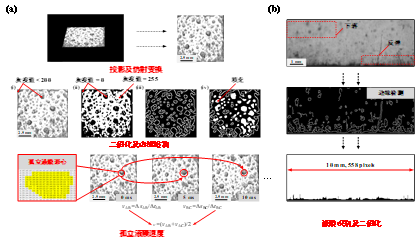
\includegraphics[scale=1.3]{figures/figure6}
	\bicaption{图像处理示意图}{Image processing diagram}\label{fig6:diagram}
\end{figure}
\begin{table}[t]
	\centering
	\bicaption{各参数误差}{Errors E of parameters} \label{}
	\begin{tabular}{m{5em}<{\centering}m{5em}<{\centering}m{5em}<{\centering}}%但由于设置了表格的整体宽度,为了使表格对齐,需要使用表达式 @{\extracolsep{\fill}}
		\toprule[2pt]
		参数 &$E^+$&$E^-$\\
		\midrule[1pt]
		δh/h&	+9.78\%&	−9.78\%\\
		${δA}_{\rm{{wet}}}$/${A}_{\rm{{wet}}}$&	+4.00\%&	0\\
		δd/d	&+2.00\%	&0\\
		δv/v	&+6.58\%&	−6.58\%\\
		Bo	&+19.62\%	&−19.62\%\\
		Ra	&+29.58\%	&−29.58\%\\
		$\rm{{Ma}_{g}}$	&+10.52\%&	−10.52\%\\
		$\rm{Ma}_{R}$	&+6.76\%&	−6.48\%\\
		Wb	&+14.72\%	&−14.59\%\\
		We	&+13.40\% &	−13.25\%\\
		Re	&+7.04\%	&−6.75\%\\	
		Re	&+7.04\%&	−6.75\%\\
		\bottomrule[2pt]
	\end{tabular}
\end{table} 

\BiChapter{MA Thesis使用指南}{Use Guide of Ph.D Dissertation}
安装配置环境与编辑器选择:使用此模板需先下载TeX Live用以配置编译环境,还需下载TeXstudio作为编辑器。当TeX Live和TeXstudio下载好后可不用管TeX Live,直接在TeXstudio中编辑运行即可。\par
打开TeXstudio,点击菜单栏里的选项按钮,选择编辑TeXstudio,在构建里将默认编辑器设置成XeLaTex,再点击菜单栏里的文件选择打开选项打开DUT文件夹里的MA Thesis.tex文件,之后点击绿色的运行按钮进行首次编译运行,最后添加自己的内容进行论文撰写。
\BiSection{此Latex论文模板使用须知}{Basic Instructions for Using Latex}
(1)知道\textbackslash chapter\{\}是章开始的意思,在{}里面填入章节名称,然后在后面写上内容即可;同理\textbackslash section\{\}和\textbackslash subsection\{\}分别对应节、次节,用法同“章”;\par
(2)知道另起一段在一段内容结束后用\textbackslash par即可达到另起一段的目的;至于换行不用管会自动换行的;\par
(3)知道在什么地方填内容,参考模板中abstract、denotation、chapter1-6、app1、app2、pub、thanks、resume去填入自己论文的内容。\par
(4)论文中的封面、原创性申明和授权书、奇偶页页眉内容填写在DUT-thesis-grd.cls文件里进行编辑,需要论文作者找到对应位置进行内容更改,具体编辑位置如下图中红框部分所示:\par
论文封面内容编辑:\par
\begin{figure}[!ht]
	\centering
	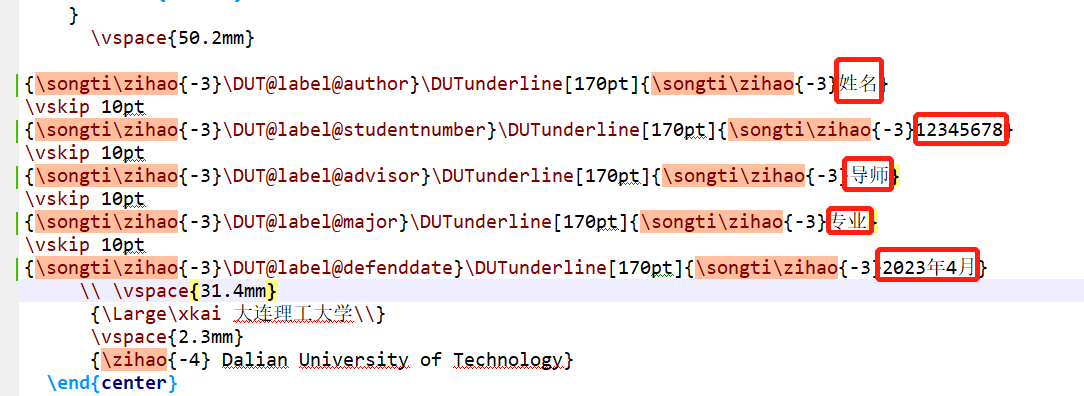
\includegraphics[width=0.9\textwidth]{figures/figure10}
	\bicaption{封面}{cover}  
\end{figure}
原创性申明和授权书内容编辑:\par
\begin{figure}[H]
	\centering
	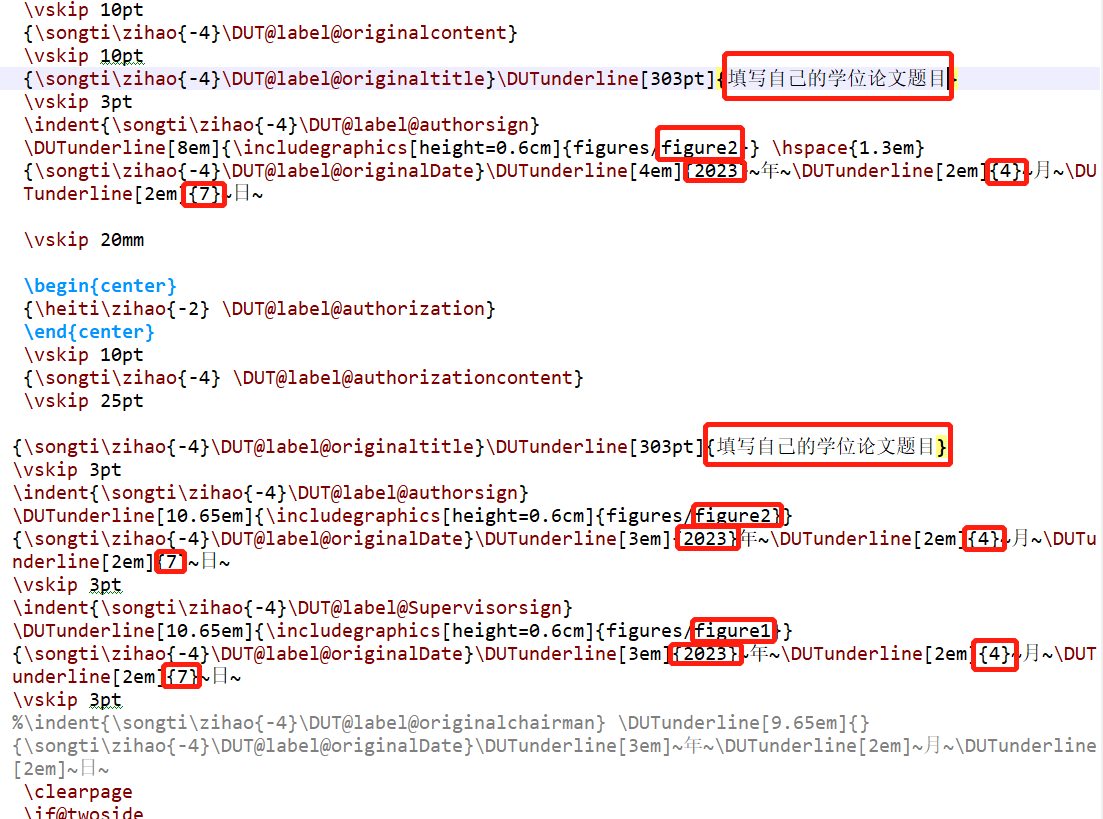
\includegraphics[width=0.8\textwidth,height=0.5\textwidth]{figures/figure11}
	\bicaption{申明}{statements}  
\end{figure}
奇偶页页眉编辑:\par
\begin{figure}[!ht]
	\centering
	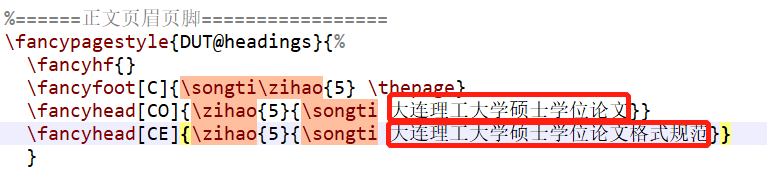
\includegraphics{figures/figure12}
	\bicaption{页眉}{header}  
\end{figure}
(5)要想用好latex进行论文写作,仅通过本文的介绍还不够,建议的学习资料如下:\url{https://github.com/BIT-thesis/LaTeX-materials}\par

 

%(其后部分无编号)
\backmatter

% 发表文章目录
%%==================================================
%% pub.tex for DUT Thesis
%% version: 0.1
%% last update: Apr 27th, 2022
%%==================================================

\begin{publications}
	\subsubsection*{\textbf{~~已发表论文}}
	\vspace{-10pt}
	\begin{enumerate}[label={[\arabic*]}]
		\item\textbf{Zhao X}, Yin Z, Zhang B*, Yang Z. Experimental investigation of surface temperature non-uniformity in spray cooling [J]. \textbf{\textsl{International Journal of Heat and Mass Transfer}}, 2020, 146: 118819. (SCI: 000500371700033, EI: 20194207543161, IF: 4.346, 本学位论文第三章) 
		\item\textbf{作者1}, 作者2, 作者3, 作者4*. 基于导热逆问题的间歇性喷雾研究, \textit{中国工程热物理学会多相流学术会议}, 2018, 北京. (本学位论文第四章)
	\end{enumerate}
	\subsubsection*{\textbf{~~待发表论文}}
	\vspace{-10pt}
	\begin{enumerate}[label={[\arabic*]}]
		\item\textbf{Zhang Q}, Chen S*, Yu H, Quan X*. Solar-driven simultaneously extracting clean water and pure NH3•H2O solution by carbonized wood. In Preparation/Under Review (本学位论文第二章)
	\end{enumerate}
	\subsubsection*{\textbf{~~发明专利}}
	\vspace{-10pt}
	\begin{enumerate}[label={[\arabic*]}]
		\item\textbf{发明人1}, 发明人2, 发明人3. 多功能一次性压舌板: 中国. 发明类别: 发明专利. 授权公告号: 92214985.2 [P], 公开(或授权)日期: 1993.04.14.
		\item\textbf{发明人1}, 发明人2. 发明人3. 气体恒温控制装置及混合气体节流系统: 中国. 发明类别: 发明专利. 授权公告号: CN 107562086 B, 授权公告日: 2020.02.14.
	\end{enumerate}	
	\subsubsection*{\textbf{~~获得奖励}}
	\vspace{-10pt}
	\begin{enumerate}[label={[\arabic*]}]
		\item “大型C/E复合材料构件高质高效加工关键技术及其工艺装备”, 机械工业科学技术奖-科技进步一等奖, 2013.10, 完成人排序: x/y(如1/3).
	\end{enumerate}
	\subsubsection*{\textbf{~~参与科研项目}}
	\vspace{-10pt}
	\begin{enumerate}[label={[\arabic*]}]
		\item 国家自然科学基金面上项目(21476037): 微细通道内液滴运动行为的调控及混合与吸收过程强化机理的研究, 2015.01 – 2018.12, 负责人: 张三.
	\end{enumerate}	
\end{publications}

% 致谢

%%==================================================
%% thanks.tex for DUT Thesis
%% version: 0.1
%% last update: Apr 27th, 2022
%%==================================================

\begin{thanks}
	学位论文中不得书写与论文工作无关的人和事(可以写家人),对导师的致谢要实事求是。\par
	对指导或协助指导完成论文的导师、资助基金或合同单位、提供帮助和支持的同志应在论文中做明确的说明并表示谢意。\par
	这部分内容不可省略。\par
\end{thanks}



\end{document}
